%
% teil2.tex -- Beispiel-File für teil2 
%
% (c) 2020 Prof Dr Andreas Müller, Hochschule Rapperswil
%
% !TEX root = ../../buch.tex
% !TEX encoding = UTF-8
%

\section{Das optimale Steuerungsproblem der Rakete \label{leo:section:optimalsteuerung}}
\rhead{Optimales Steuerungsproblem}

Der Raketenaufstieg ist ein klassisches Beispiel für ein \textit{optimales Steuerungsproblem}. 
Im Gegensatz zu Standard-Variationsproblemen, bei denen eine Funktion gesucht wird, die ein bestimmtes Integral extremal macht, erfordert das Raketenproblem die Steuerung eines Systems, um ein Ziel wie die Minimierung des Treibstoffverbrauchs oder das Erreichen einer bestimmten Endgeschwindigkeit zu erreichen. Dabei wird das System durch Differentialgleichungen beschrieben, die den physikalischen Gesetzen folgen, und die Steuerung erfolgt über gezielte Eingaben wie den Schubwinkel oder die Schubkraft.

Ziel des Raketenaufstiegs ist es, eine Umlaufbahn zu erreichen, während Verluste durch Schwerkraft, Luftwiderstand und Steuerung minimiert werden. 
Diese Verluste hängen jedoch von der Steuerfunktion \( u(t) \) ab, die dynamisch angepasst werden muss. 
Im Unterschied zu klassischen Variationsproblemen, bei denen die Lösung nur von den Zustandsvariablen \( x(t) \) abhängt, wird hier die Steuerung \( u(t) \) als eigenständige Funktion betrachtet, die die Dynamik der Zustandsgrößen beeinflusst.

\subsection{Warum das Problem nicht mit einer üblichen Lagrange-Funktion lösbar ist}

In klassischen Variationsproblemen wird eine Lagrange-Funktion \(L(x, \dot{x})\) verwendet, die von den Zustandsvariablen \(x(t)\) und deren zeitlichen Ableitungen \(\dot{x}(t)\) abhängt, um den optimalen Pfad eines Systems zu berechnen. 
Diese Probleme lassen sich häufig analytisch durch die Euler-Lagrange-Gleichungen lösen.

Das Raketenproblem ist jedoch komplexer. 
Hier müssen Steuerfunktionen wie der Schubwinkel oder die Schubkraft dynamisch angepasst werden, um äußeren Bedingungen wie der Schwerkraft oder dem Luftwiderstand zu begegnen. 
Die alleinige Optimierung der Zustandsgrößen \(x(t)\) reicht nicht aus, da die Steuerfunktion \(u(t)\) aktiv in die Dynamik des Systems eingreift. 
Daher muss das Problem als \textit{optimales Steuerungsproblem} betrachtet werden, bei dem sowohl die Zustandsgrößen \(x(t)\) als auch die Steuergrößen \(u(t)\) optimiert werden, um den Treibstoffverbrauch zu minimieren und die gewünschten Endbedingungen zu erreichen.

\subsection{Identifizierung des optimalen Steuerungsproblems}

Das Steuerungsproblem lässt sich durch eine Differentialgleichung des Systems beschreiben:
\[
\dot{x} = f(x,u),
\]
wobei \(x(t)\) den Zustandsvektor der Rakete (z.\,B. Position, Geschwindigkeit) und \(u(t)\) die Steuerfunktionen (z.\,B. Schubwinkel) darstellt. 
Die Funktion \(f(x,u)\) beschreibt die Dynamik der Rakete, die durch Schwerkraft, Luftwiderstand und Schub beeinflusst wird.

Ziel des optimalen Steuerungsproblems ist es, die Steuerfunktionen \(u(t)\) so zu wählen, dass die Rakete mit minimalem Treibstoffverbrauch und unter Einhaltung bestimmter Randbedingungen (z.\,B. Umlaufbahngeschwindigkeit) in den Orbit gelangt. 
Dies lässt sich durch ein Kostenfunktional ausdrücken:
\[
J(u) = \int_{t_0}^{t_f} L(x(t), u(t))\, dt + K(x(t_f)),
\]
wobei \(L(x(t), u(t))\) die Laufkostenfunktion darstellt, die Treibstoffverbrauch und Verluste beschreibt, und \(K(x(t_f))\) die Endkostenfunktion, die Bedingungen am Endpunkt wie z.\,B. die Geschwindigkeit und Höhe im Orbit berücksichtigt.

\subsection{Kostenfunktional und Steuerverluste}

In Kapitel \ref{buch:hamiltonjacobi:section:oc} wird das optimale Steuerungsproblem als Minimierungsproblem eines Integrals dargestellt, das die Steuerkosten über die Zeit aufintegriert. 
Für das Raketenproblem bedeutet dies, dass der Treibstoffverbrauch minimiert werden soll, während die Randbedingungen eingehalten werden. 
Die Lagrange-Funktion \(L(x(t), u(t))\) hängt in diesem Fall von der Position, Geschwindigkeit der Rakete und den Steuergrößen ab.

Ein wichtiger Aspekt der Steuerung sind die \textit{Steuerverluste}, die durch die Kursänderung der Rakete entstehen. Diese Verluste wurden in der Formel \eqref{leo:aufstiegsgleichung} beschrieben:
\[
v_f = v_* \ln \left(\frac{m_0}{m_f}\right) - 2F_* \int_0^{t_f} \frac{\sin^2\left(\frac{\alpha}{2}\right)}{m} \, dt - \dots
\]
Hier beschreibt der Term \(2F_* \int_0^{t_f} \frac{\sin^2\left(\frac{\alpha}{2}\right)}{m} \, dt\) die Steuerverluste, die minimiert werden sollen, um den Treibstoffverbrauch zu verringern.

\subsection{Hamilton-Funktion und das Pontryagin’sche Minimum-Prinzip}

Um dieses optimale Steuerungsproblem zu lösen, wird das Pontryagin'sche Minimum-Prinzip verwendet, das in Kapitel \ref{buch:hamiltonjacobi:oc:subsection:minimum} eingeführt wurde. Dazu wird eine \textit{Hamilton-Funktion} \(H(x,u,p)\) definiert:
\[
H(x,u,p) = p \cdot f(x,u) + L(x,u),
\]
wobei \(p(t)\) ein Vektor von Lagrange-Multiplikatoren ist, die die Sensitivität des Kostenfunktionals gegenüber den Zustandsgrößen beschreiben. Die Aufgabe besteht nun darin, eine Steuerfunktion \(u(t)\) zu finden, die die Hamilton-Funktion minimiert:
\[
u_*(t) = \operatorname{argmin}_{u \in \mathbb{R}} H(x_*(t), u, p_*(t)).
\]
Diese Bedingung garantiert, dass die Steuerstrategie den minimalen Treibstoffverbrauch erfordert, um die vorgegebene Bahn zu erreichen.

\subsection{Zusammenfassung der Komponenten}
%
%Das optimale Steuerungsproblem der Rakete lässt sich in folgende wesentliche Komponenten unterteilen:
%
%\begin{itemize}
%	\item \textbf{Systemgleichung}: Die Dynamik der Rakete wird durch eine Differentialgleichung beschrieben, bei der die Zustandsgrößen \(x(t)\) und die Steuergrößen \(u(t)\) interagieren.
%	\item \textbf{Kostenfunktional}: Das Kostenfunktional beschreibt die zu minimierenden Verluste, einschließlich des Treibstoffverbrauchs und der Verluste durch Schwerkraft und Luftwiderstand. Es besteht aus einem Integral über die Laufkosten und einem Randterm, der die Endbedingungen festlegt.
%	\item \textbf{Hamilton-Funktion}: Die Hamilton-Funktion kombiniert die Dynamik des Systems mit dem Kostenfunktional und dient als Grundlage für die Optimierung der Steuerfunktion. Das Pontryagin'sche Minimum-Prinzip hilft, die optimale Steuerfunktion zu finden.
%\end{itemize}

Der Raketenaufstieg lässt sich als \textit{optimales Steuerungsproblem} formulieren, bei dem die Steuerfunktion \( u(t) \) die Bahnfunktionen \( x(t) \) beeinflusst. 
Das Ziel ist es, ein Kostenfunktional zu minimieren, welches den Treibstoffverbrauch sowie andere Verlustmechanismen, wie Steuer- und Schwerkraftverluste, umfasst.

\subsubsection{Steuerfunktionen \( u(t) \)}

Die Steuerfunktion \( u(t) \) beschreibt die Parameter, die aktiv verändert werden können, um den optimalen Aufstieg zu erreichen. 
In unserem Fall ist die Steuerfunktion \( u(t) \) der \textit{Schubwinkel} \( \alpha(t) \), der den Neigungswinkel des Schubvektors der Rakete relativ zur momentanen Flugrichtung angibt. 
Diese Steuerung erfolgt durch das Pitch-Manöver, das in Abschnitt \ref{leo:section:variabeln} eingeführt wurde. 
Die Optimierung des Steuerwinkels \( \alpha(t) \) zielt darauf ab, die Verluste durch Schwerkraft und Luftwiderstand zu minimieren, während die Rakete die angestrebte Umlaufbahn erreicht.

Die entsprechende Bewegungsgleichung für die Änderung des Flugwinkels \( \dot{\gamma} \), die in Abschnitt \ref{leo:section:beweungsgleichungen} behandelt wurde, lautet
\[
\dot{\gamma} = \frac{1}{v} \left( \frac{F_*}{m} \sin \alpha + \frac{L}{m} - \left( g - \frac{v^2}{r} \right) \cos \gamma \right),
\]
wobei \( \alpha(t) \) die Steuerfunktion \( u(t) \) darstellt.

\subsubsection{Bahnfunktionen \( x(t) \)}
Die Bahnfunktionen \( x(t) \) umfassen die \textit{Position} und \textit{Geschwindigkeit} der Rakete zu jedem Zeitpunkt. 
Diese Größen werden durch den Zustandsvektor \( x(t) \) beschrieben, der aus den Komponenten Höhe \( h(t) \), horizontaler Position \( x(t) \), Geschwindigkeit \( v(t) \) und Flugwinkel \( \gamma(t) \) besteht:

\[
x(t) = \begin{pmatrix} h(t) \\ x(t) \\ v(t) \\ \gamma(t) \end{pmatrix}.
\]

Die Dynamik dieses Systems wird durch die Bewegungsgleichungen beschrieben, die in Abschnitt \ref{leo:section:beweungsgleichungen} eingeführt wurden. 
Diese beinhalten beispielsweise die Änderungsraten der Höhe und der horizontalen Position der Rakete
\[
\dot{h} = v \sin \gamma, \quad \dot{x} = v \cos \gamma
\].

\subsubsection{Kostenfunktional}
Das Kostenfunktional beschreibt das Ziel der Optimierung. Für das Raketenproblem ist dies der Treibstoffverbrauch und die Verluste, die während des Aufstiegs minimiert werden sollen. 
Das Kostenfunktional lässt sich durch ein Integral der Form
\[
J(u) = \int_{t_0}^{t_f} L(x(t), u(t)) \, dt
\]
darstellen, wobei \( L(x(t), u(t)) \) die \textit{Laufkostenfunktion} darstellt, die den Treibstoffverbrauch, Steuerverluste und Schwerkraftverluste beschreibt.

Wie in Abschnitt \ref{leo:section:aufstiegsgleichung} eingeführt, werden diese Verluste durch folgende die Gleichung
\[
v_f = v_* \ln \left(\frac{m_0}{m_f}\right) - 2F_* \int_0^{t_f} \frac{\sin^2\left(\frac{\alpha}{2}\right)}{m} \, dt - \dots
\]
beschrieben. Hierbei müssen die Steuerverluste, die durch den Schubwinkel \( \alpha(t) \) beeinflusst werden, minimiert werden.

\subsubsection{Randbedingungen}
Die Randbedingungen legen fest, welche Anfangs- und Endwerte für die Rakete während des Aufstiegs gelten. Zu Beginn des Fluges (bei \( t_0 \)) startet die Rakete vom Boden, was durch die Anfangsbedingungen
\[
h(t_0) = 0, \quad v(t_0) = 0
\]
festgelegt ist. 
Am Ende des Fluges (bei \( t_f \)) muss die Rakete eine vorgegebene Höhe \( h(t_f) \) sowie die Endgeschwindigkeit \( v(t_f) \) erreichen
\[
h(t_f) = H, \quad v(t_f) = v_{orbit}
\]
um in die Umlaufbahn zu gelangen.
Diese Bedingungen stellen sicher, dass die Rakete den gewünschten Orbit erreicht, während das Kostenfunktional \( J(u) \) minimiert wird.
Die Randbedingungen, wie die gewünschte Höhe und Geschwindigkeit, wurden in Abschnitt \ref{leo:section:raketengleichung} in Verbindung mit der Orbitalmechanik behandelt.

Das Steuerungsproblem der Rakete zeigt die Komplexität der Steuerung in der Raumfahrt auf, bei der verschiedene Einflüsse wie Schwerkraft und Luftwiderstand berücksichtigt werden müssen. Eine genaue Lösung dieses Problems erfordert numerische Methoden, um die optimalen Steuerfunktionen zu berechnen.

\section{Die optimale Flugbahn}

Urlich Walter sagt in seinem Buch zur Lösung der optimalen Flugbahn folgendes: ''Letztendlich basiert eine gute Aufstiegsoptimierung auf ausgefeilter Software, auf der Kenntnis der grundlegenden Aufstiegsmanöver, aber auch auf den Fähigkeiten erfahrener Flugmechaniker und auf Versuch und Irrtum.``
Die Flugbahn ist von so vielen Faktoren abhängig, dass immer noch nicht die genau Flugbahn berechnet werden kann. 
Oder wie der Witz für viele schwierige Aufgaben in der Wissenschaft geht: ''In 10 Jahren sind wir dann so weit.``

\begin{figure}
	\centering
	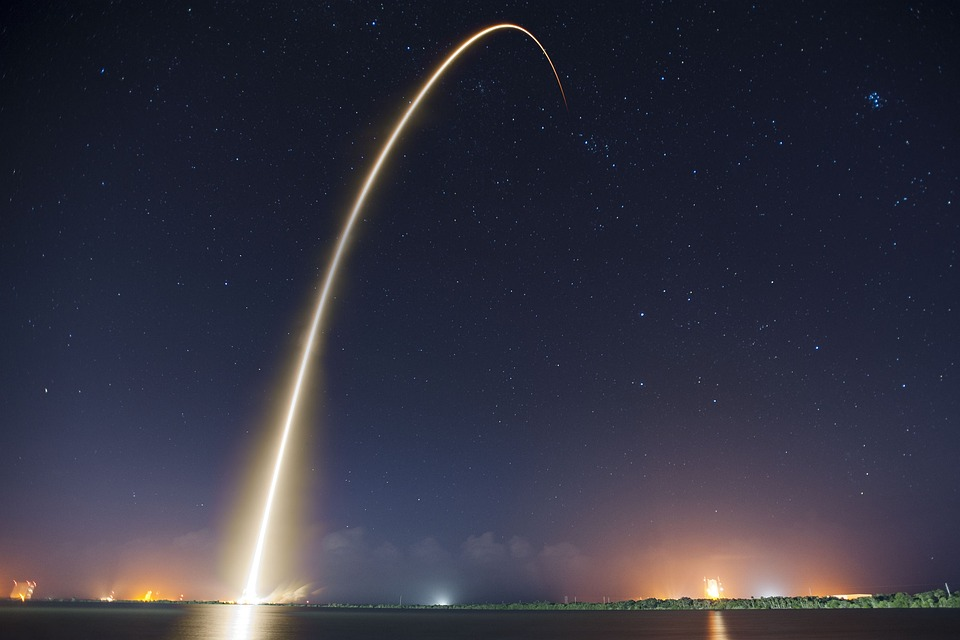
\includegraphics[width=0.9\linewidth]{papers/leo/Grafiken/rocket-launch}
	\caption{Langzeit Beleuchtung eines Raketen Starts.}
	\label{fig:rocket-launch}
\end{figure}


